\documentclass[12pt]{article}
\usepackage[left=3.5cm,right=2cm,top=2.5cm,bottom=2.5cm]{geometry}
\usepackage[T1]{fontenc}
\usepackage[utf8]{inputenc}
\usepackage{tgpagella}
\usepackage{enumerate}
\usepackage{url}
\usepackage{multirow}
\usepackage{longtable}
\usepackage{polski}
\usepackage{graphicx}
\usepackage{float}
\usepackage{color}
\usepackage{amsmath}
\usepackage{longtable}
\usepackage{tabularx}
\usepackage{ltablex,booktabs}
\usepackage{amssymb}
\usepackage{rotating}
\usepackage{subfigure}
\usepackage{float}
\usepackage{tabu}
\usepackage{caption}
\usepackage{footnote}
\usepackage{xspace}
\usepackage{mathpazo}
\usepackage[table]{xcolor}
\usepackage[justification=centering]{caption}
\graphicspath{ {images/} }

\pagestyle{empty}

\title{\LARGE{Uniwersytet Wrocławski}\\
\Large{Wydział Matematyki i Informatyki}\\
\large{Kierunek: Informatyka}}

\date{}

\begin{document}
\pagestyle{empty}

\begin{titlepage}
\maketitle
\thispagestyle{empty}


\begin{center}
\author{\LARGE{Adrian Mularczyk}}
\vspace{30pt}

\huge{\textbf{Stworzenie wydajnego wzorca wstrzykiwania zależności dla złożonych grafów zależności}}
\vspace{50pt}
\end{center}

\begin{flushright}
\large{Praca wykonana pod kierunkiem}
\large{dr. Wiktora Zychli}
\end{flushright}

\vfill
\begin{center}
\begin{large}
Wrocław, 2016
\end{large}
\end{center}
\end{titlepage}

\setlength{\parindent}{0pt}	%usunięcie wcięć
\setlength{\parskip}{1.5ex} 
\renewcommand*{\figurename}{Rys.}
\renewcommand*{\tablename}{Tab.} 
\renewcommand{\captionsize}{\small}


\clearpage

\tableofcontents



\clearpage

\section{Wstęp}
\subsection{Cel pracy}
Wstrzykiwanie zależnośc jest wzorcem projektowym, który pozwala na tworzenie kodu o luźniejszych powiązaniach, łatwiejszego w testowaniu i modyfikacji. Najbardziej popularnymi implementacjami tego wzorca w języku C\# są Unity i Ninject. Celem niniejszej pracy magisterskiej jest stworzenie wydajnej implementacji tego wzorca dla złożonych grafów zależności. Do tego celu zostanie wykorzystana funkcjolanosci z przestrzeni nazw Reflection.Emit. W tej pracy zostaną przedstawione dwa rozwiązania.

\subsection{Układ pracy}
Poza wstępem i podsumowaniem praca składa się jeszcze z trzech rozdziałów. W pierwszym znajduje się opis teoretyczny czym jest wstrzykiwanie zależności. Drugi rozdział opisuje moją implementację tego wzorca. Trzeci rozdział skupia się na testach wydajnościowych, w którym porównuję moją implementację z kilkoma najbardziej popularnym i kilkoma najszybszymi implementacjami.



\clearpage

\section{Wstrzykiwanie zależnosci}
\subsection{Wstęp}
Jest to zbiór zasad projektowania oprogramowania i wzorców, które pozwalają nam rozwijać luźno powiązany kod \cite{dependency_injection}.\\
Jakiemu celowi ma służyć wstrzykiwanie zależności? Wstrzykiwanie zależnści nie jestem celem samym w sobie, raczej jest to środek do celu. Ostatecznie celem większości technik programowania jest dostarczenie jak najwydajniej działającego oprogramowania. Jednym z aspektów tego jest napisanie utrzymywalnego kodu.\\
O ile nie pisze się prototypu lub aplikacji, które nigdy nie mają kolejnych wersji (kończą się na wersji 1), to wkrótce będzie trzeba zająć się utrzymaniem i rozwijaniem istniejącego kodu. Aby być w stanie pracować wydajnie z takim kodem bazowym, musi on być jak najlepiej utrzymywalny.\\
Wstrzykiwanie zależności jest niczym więcej niż techniką, która umożliwia luźne powiązania, a luźne powiązania sprawiają, że kod jest rozszerzalny i łatwy w utrzymaniu. \cite{dependency_injection}\\
Wstrzykiwanie zależności może odbywać się na 3 sposoby\\
- wstrzykiwanie przez konstruktor (główna i najbardziej popularna)\\
- wstrzykiwanie przez metodę\\
- wstrzykiwanie przez propercję\\

\subsection{Implementacje przemysłowe}
Na rynku jest wiele implementacji wstrzykiwania zależności. Przedstawię tutaj kilka najbardziej popularnych (według ilości pobrań z NuGet) oraz kilka najszybszych (według rankingu na stronie: http://www.palmmedia.de/Blog/2011/8/30/ioc-container-benchmark-performance-comparison). Dane zostały wzięte z dnia 21-02-2017.\\
Najbardziej popularne:
\begin{itemize}
	\item Unity (4.0.1) - ponad 5.2 mln pobrań
	\item NInject (3.2.2) - ponad 4.0 mln pobrań
	\item Autofac (4.3.0) - ponad 3.7 mln pobrań
	\item StructureMap (4.4.3) - ponad 1.6 mln pobrań
	\item Windsor (3.4.0) - ponad 1.4 mln pobrań
\end{itemize}
Najszybsze:
\begin{itemize}
	\item Grace (5.1.0)
	\item DryIoc (2.10.1)
	\item LightInject (5.0.1)
	\item SimpleInjector (3.3.2)
\end{itemize}



\clearpage

\section{Implementacja}
Kod źródłowy programu jest dostępnym w repozytorium pod adresem: \url{https://github.com/amularczyk/NiquIoC}\\
Znajduje się tam też również kod programu, który posłużył do wykonania testów wydajnościowych, a także ta praca napisana w języku LateX i wszystkie obrazki.

\subsection{Środowisko pracy}
Prac oraz wszystkie testy powstały na komputerze z parametrami:
\begin{itemize}
	\item Intel Core i7-4720HQ (2.60GHz)
	\item 12 GB pamięci RAM
	\item Dysk SSD
\end{itemize}
Narzędzia użyte do stworzenia pracy i testów:
\begin{itemize}
	\item {\color{red} System operacyjny Windows 10 Pro}
	\item .Net Framework w wersji 4.6.1
	\item Visual Studio 2015 Comunnity
	\item ReSharper
	\item Dia
\end{itemize}
Testy zostały wykonane we frameworku XUnity, który jest wbudowany w Visual Studio.\\
Rozwiązanie opiera się na użyciu operacji z przestrzeni nazw System.Reflection.Emit.

{\color{red}
\subsection{Microsoft Intermediate Language}
Microsoft Intermediate Language - MSIL (w skrócie IL) to język pośredni do którego kod C\# jest kompilowany. Język ten pozwala na komunikację między aplikacjami napisanymi na platformie .Net, a systemem operacyjnym. Jest on jądrem tej platformy.
}


{\color{red}
\subsection{Reflection.Emit}
Przestrzeń nazw Reflection.Emit pozwala ona na stworzenie ciągu operacji w języku IL, a następnie zapamiętaniu ciągu tych operacji jako delegat. Za każdym razem, gdy ten delegat zostanie wywołany, to wykona się ciąg wczeniej zdefiniowanych operacji IL.
}

\subsection{Architektura}
Aplikacja składa się z 1 projektu i 4 projektów na potrzeby testów. Aplikacja jest skomplikowana i aby mieć pewność, że działa w pełni dobrze zostało stworzone {\color{red} ponad 1000} testów jednostkowych.\\

W wykonanej implementacji został stworzony interfejs IConatiner, który definiuje operacje, jakie powinny się znaleźć w każdym kontenerze:
\begin{itemize}
	\item IContainerMember RegisterType<T>() where T : class
	\item IContainerMember RegisterType<TFrom, TTo>() where TTo : TFrom
	\item IContainerMember RegisterType<T>(Func<object> objectFactory) where T : class
	\item IContainerMember RegisterInstance<T>(T instance)
	\item T Resolve<T>(ResolveKind resolveKind)
	\item void BuildUp<T>(T instance, ResolveKind resolveKind)
\end{itemize}
Pierwsze 4 metody służą do rejestracji typów do kontenera. W pierwszej metodzie możemy zarejestrować zwykłe klasy. W drugiej interfejsy i klasy, które implementują dany interfejs. W trzeciej metodzie rejestrujemy klasę jako fabrykę obiektów - funkcję, która ma nam zwrócić pożądany obiekt. W czwartej możemy zarejestrować konkretną instancję danej klasy. W mojej implementacji kontenera każdy typ może być zarejestrowany tylko raz - ponowna rejestracja tego samego typu nadpisuje istniejącą rejestrację.\\
Każda z tych czterech pierwszy metod zwraca interfejs IContainerMember, który umożliwia nam zarejestrowanie danej klasy lub interfejsu z określonym menadżerem czasu życia. Jest to po to, ponieważ dla różnych przypadków biznesowych możemy potrzebować, aby obiekt danego typu miał konretny czas życia. Ten interfejs daje nam możliwość ustawienia czasu życia na:
\begin{itemize}
	\item Singleton
	\item Transient
	\item PerThread
	\item PerHttpContext
	\item Custom (dowolna, stworzona przez użytkownika implementacja interfejsu IObjectLifetimeManager)
\end{itemize}
W mojej implementacji kontenera każdy typ domyślnie ma czas życia Transient.\\
Interfejs IObjectLifetimeManager zawiera w sobie następujące metody:
\begin{itemize}
	\item  Func<object> ObjectFactory { get; set; }
	\item object GetInstance()
\end{itemize}
Pierwsza z nich służy to ustawienia fabryki, która zwraca obiekt. Druga służy do zwracania obiektu przy użyciu fabryki. W zależności od konkretnego czasu życia, to obiekt zwracany z metody GetInstance może być zwsze ten sam, zwsze różny albo ten sam tylko dla określonych sytuacji (np. ten sam dla tego samego wątku albo ten sam dla tego samego żądania).\\

Metoda piąta - Resolve, to główna metoda. Register można nazwać sercem kontenera, a Resolve mózgiem. Odpowiada ona za stworzenie i zwrócenie obiektu odpowiedniego typu. W mojej pracy zaproponowałem dwa rozwiązania - PartialEmitFunction i FullEmitFunction, dlatego ta metoda jako parametr przyjmuje wartość enuma ResolveKind.\\
Szósta metoda to taki dodatek - gdy mamy stworzony obiekt, ale nie jest w pełni uzupełniony, wtedy możemy go zbudować (używająć odpowiednio PartialEmitFunction lub FullEmitFunction). Z tą metodą są powiązane bezpośrednio dwa pojęcia - wstrzykiwanie przez metodę i wstrzykiwanie przez propercję. Do tego celu zostały stworzone dwa atrybuty:
\begin{itemize}
	\item DependencyMethod (dla metod)
	\item DependencyProperty (dla propercji)
\end{itemize}
Podczas operacji BuildUp uzupełniane są wywoływane wszystie metody i propercje, które mają te atrybuty. BuildUp jest również wykonywany podczas operacji Resolve.\\
Warto tutaj odnotować, że ze względu na szczegóły implementacyjne tylko jedno z moich rozwiązań wspiera operację BuildUp - PartialEmitFunction. W FullEmitFunction ta funckonalność nie została zaimplementowana. Jest to spowodowane skomplikowaniem FullEmitFunction i małą potrzebą biznesową używania operacji BuildUp.\\

W aplikacji istnieje również atrybut DependencyConstrutor. Można go użyć przy definicji konstruktora danej klasy. Obiekty danej klasy tworzy się przy użyciu konstruktora. Dana klasa może mieć kilka konstruktorów. W mojej implementacji stworzyłem logikę wyboru konstruktora przy pomocy którego ma zostać stworzony obiekt. Jeśli jest kilka konstrutkrów, odpowiedni jest wybierany w następującej kolejności:
\begin{itemize}
	\item Konstruktor z atrybutem DependencyConstrutor
	\item Konstrutkro z największą liczbą parametrów
\end{itemize}
Jeśli jest kilka konstrutkrów z atrybutem DependencyConstrutor albo kilka z największą liczbą parametrów, to rzucany jest wyjątek.\\


\subsection{Rozwiązanie}
Aby kontener działał wydajnie dla złożonych grafów zależności, należy jak najwięcej informacji przechowywać w cache i należy to robić mądrze. W tym celum wykorzystałem Reflection.Emit, aby zapamiętać ciągu operacji niezbędnych do stworzenia obiektu nowej klasy (na potrzeby metody Resolve). Wykorzystałem to na dwa sposoby, które zostały opisane poniżej.


\subsection{Rozwiązanie 1 - PartialEmitFunction}
W pierwszym rozwiązanu, które nazwałem PartialEmitFunction tworzę delegata z wykorzystaniem Reflection.Emit. Delegat ten jako parametr przyjmuje listę obiektów, które są potrzebne do stworzenia obiektu danej klasy wykorzystując odpowiedni konstruktor. Jeśli kontener do stworzenia obiektu danej klasy wybrał konstruktor bezparametrowy, to do takiego delegata trafi pusta lista. Jeśli natomiast został wybrany konstruktor, który w parametrze np. potrzebuje obiektu klasy A i B, to do delegata zostanie przekazana lista zawierająca obiekt klasy A i B w kolejności takiej, jakiej są one zdefiniowane z konstruktorze.\\
Pseudokod tego rozwiązana wygląda następująco:
\begin{enumerate}
	\item Dla każdego argumentu umieść ten argument na stosie
	\item Na stosie umieść konstruktor docelowego typu
	\item Wywołaj konstrutkor i stworzony obiekt umięść na szczycie stosu
	\item Zwróć obiekt ze szczytu stosu
\end{enumerate}
To rozwiążanie nazwał "Partial", ponieważ tylko część operacji niezbędnych do stworzenia obiektu jest zakodowanych w języku IL (pobranie argumentów i stworzenie obiektu). W tym rozwiążaniu musimy wcześniej stworzyć obiekty, które są potrzebne do stworzenia docelowego obiektu.\\
To rozwiązanie powinno lepiej się sprawdzać w sytuacjach, gdy wierzchołki w grafie zależnoci czesto się powtarzają i w aplikacji nie wykonujemy zbyć często operacji "Resolve".


\subsection{Rozwiązanie 2 - FullEmitFunction}
W drugim rozwiążaniu, które nazwałem FullEmitFunction tworzę delegata bezparametrowego. Sam tworzy on wszystkie obiekty, które są mu potrzebne do stworzenia docelowego obiektu. Działa on rekurencyjnie i najpierw na stosie umieszcza wszystkie operacje niezbędne do stworzenia obiektu danego typu, a następnie tworzy docelowy obiekt.\\
Pseudokod tego rozwiązania wygląda następująco:
\begin{enumerate}
	\item Czy konstruktor danego typu potrzebuje jakiś argument?
	\begin{enumerate}
		\item Tak - Dla każdego parametru konstruktora wywołaj rekurencyjnie funkcję z argumentem wejściowym jako typ parametru.
		\item Nie - Idź dalej.
	\end{enumerate}
	\item Na stosie umieść konstruktor docelowego typu
	\item Wywołaj konstrutkor i stworzony obiekt umięść na szczycie stosu
	\item Zwróć obiekt ze szczytu stosu
\end{enumerate}
Jak łatwo zauważyć, to rozwiązanie jest pełne ("Full"), ponieważ wszystkie niezbędne obiekty zostaną stworzonę przy użyciu IL w jednej metodzie.\\
To rozwiązanie powinno lepiej się sprawdzić w sytuacjach, gdy wierzchołki w grafie zależności rzadko się powtarzają i w aplikacji dużo razy wykonujemy operację "Resolve".



\clearpage

\section{Testy wydajnościowe}
Do przeprowadzania testów wydajnościowych stworzyłem osobną aplikację w której zaimplementowałem 3 przypadki testowe (przypadek testowy A, przypadtek testowy B i przypadtek testowy C). Każdy z przypadków testowych sprawdza szybkość wykoniania operacji "Resolve" dla różnych rejestracji (operacji Register).\\
Każdy z przypadków testowych wykonuje następujące testy:
\begin{itemize}
	\item register as Singleton
	\item register as Transient
	\item register as PerThread (dla niektórych przemysłowych implementacji - PerScope)
\end{itemize}
Każdy z testów dla każdego kontenera był uruchamiany w osobnym procesie. Każdy test był uruchamiany 100(?) razy, a w wynikach zostały przedstawione następujące czasy: minimalny,  maksymalny i średni.


\subsection{Przypadek testowy A}
\subsubsection{Opis}
W tym teście mamy zdefiniowanych 11 typów i każdy z nich przymuje w konstruktorze od jeden mniej parametr mniej niż typ poprzedni. Typem głównym, a zarazem typem o największej licznie parametrów, jest typ "TestA". Przyjmuje on w konstruktorze 10 parametrów, kolejno następujących typów: "TestA0", "TestA1", "TestA2", "TestA3", "TestA4", "TestA5", "TestA6", "TestA7", "TestA8", "TestA9". Każdy z tych 10 typów w konstruktorze przyjmuje tyle obiekt, jaki ma numerek w nazwie (czyli obiekt typu "TestA0" ma konstruktore bezparametrowy, obiekt typy "TestA1" ma konstuktor z jednym parametrem; i tak dalej aż do typu "TestA9", który ma konstruktor z dziewięcioma parametrami). Każdy z tych typów jako parametry w konstruktorze przyjmuje kolejne obiekty typów z niższym numerkiem (czyli obiekt typu "TestA1" w konstruktorze przyjmuje parametr typu "TestA0", obiekt typu "TestA2" przymuje w konstruktorze obiekty typu "TestA0" i "TestA1";  i tak dalej aż do typu "TestA9", który w konstruktorze przyjmuje parametry z typami od "TestA0" do "TestA8").\\

\begin{figure}[h]
	\begin{center}
  		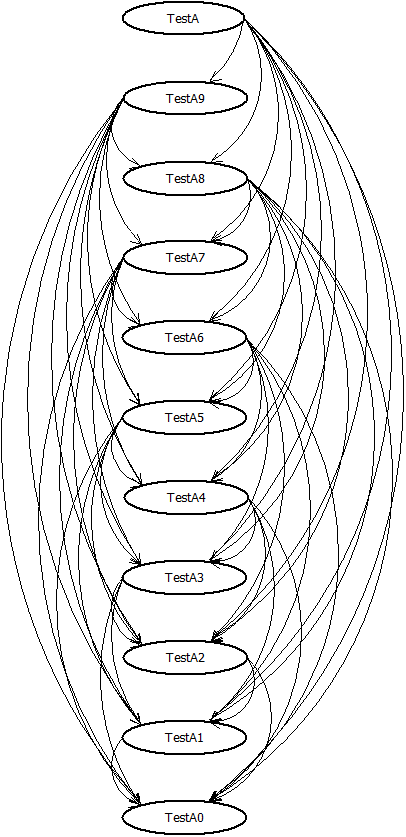
\includegraphics[height=12cm]{TestA.png}
  		\caption{Graf zależności dla testu A.}
  		\label{fig:testA}
	\end{center}
\end{figure}

Łatwo wywnioskować z Rys. \ref{fig:testA}, że tworząc obiekty poszczególnych typów ilość tworzonych obiektów rośnie dwukrotnie:
\begin{itemize}
	\item TestA0 - 1 obiekt,
	\item TestA1 - 2 obiekty (obiekt typu TestA1 i obiekt typu TestA0),
	\item TestA2 - 4 obiekty (obiekt typu TestA2, obiekt typu TestA1 - 2 obiekty, obiekt typu TestA0 - 1 obiekt),
	\item TestA3 - 8 obiektów (obiekt typu TestA3, obiekt typu TestA2 - 4 obiekty, obiekt typu TestA1, obiekt typu TestA0),
	\item TestA4 - 16 obiektów,
	\item TestA5 - 32 obiektów,
	\item TestA6 - 64 obiektów,
	\item TestA7 - 128 obiektów,
	\item TestA8 - 256 obiektów,
	\item TestA9 - 512 obiektów,
	\item TestA - 1 024 obiektów.
\end{itemize}
Zatem tworząc obiekt typu TestA, tworzymy: 1 obiekt typu TestA, 1 obiekt typu TestA9, 2 obiekty typu TestA8, 4 obiekty typu TestA7, 8 obiektów typu TestA6, 16 obiektów typu TestA5, 32 obiektów typu TestA4, 64 obiektów typu TestA3, 128 obiektów typu TestA2, 256 obiektów typu TestA1 i 512 obiektów typu TestA0.

\subsubsection{Wyniki dla Singleton}
Najlepiej poradziły sobie najpopularniejsze kontenery - Windsor i Aurofac. Kontener NiquIoCPartial uplasował się na 3 miejscu. Najsłabiej poradził sobie kontroler StructureMap i Unity.

\subsubsection{Wyniki dla Transient}
W tym teście ważne są nie tylko poszczególne czasy, ale jak i również wzrostu czasu wykonania wraz ze wzrostem ilości operacji.\\
Gdy mamy tylko 1 operację najlepiej radzi sobie Autofac, a zaraz za nim NiquIoCPartial i Windsor. Najsłabiej DryIoc i SimplyInjector.\\
Gdy mamy 10 operacji znacząco najlepiej radzi sobie NiquIoCPartial (ponad dwa razy lepiej niż drugi Autofac). Kolejne miejsca należą do NiquIoCFull i LightInject. Pozostałe kontenery miały podobne, dużo słabsze czasy. Najgorzej poradził sobie Ninject, który czas miał ponad 5 razy większy niż kontener z przedostatnim czasem (Windsor).\\
Gdy mamy 100 operacji na prowadzenie wysuneły się mniej popularne kontenery, które prawdopodobniej mają najlepsze cachowanie. Kolejne miejsca to: NiquIoCFull, LightInject i SimpleInjector. Najsłabiej w tym przypadku poradziłysobie Ninject, Windsor, Unity i Autofac.\\
Dla przypadku z 1000 operacji do czołówki dołączył DryIoc (czasy zbliżone do SimpleInjector). Na pierwszym miejscu wciąż pozostaje NiquIoC. Pozostałe kontenery mają czasy od kilka do kilkanaście razy gorsze.\\
Warto tutaj zaznaczyć, że najmniejszy wzorst czasu miały kontenery NiquIoCFull, LightInject, DryIoc, SimpleInjector oraz Grace.

\subsubsection{Wyniki dla PerThread}
Czasy dla tego przypadku powinny być zbliżone do czasów dla Singleton, ponieważ wszystko było uruchamiane w jednym wątku, więc powinno się zachowywać jak singleton. Niestety prawie połowa kontenerów sobie z tym nie poradziła. Czasy zbliżone do czasów dla Singletona posiadają jedynie: Autofac, Ninject, NiquIoCPartial, NiquIoCFull, StructureMap, Unity i Windsor. Czasy dla pozostałych kontrolerów są od kilka do nawet kilkadziesiąt razy większe niż dla Singleton.\\
Tak samo jak w przypadku Signleton najlepiej poradziły sobie najpopularniejsze kontenery - Windsor i Aurofac. Kontener NiquIoCPartial uplasował się na 3 miejscu. Najsłabiej poradził sobie kontroler LightInject i DryIoc.


\subsection{Przypadek testowy B}
\subsubsection{Opis}
W tym teście mamy zdefiniowanych 51 typów. 10 z tych typów ma konstruktor bezparametrowy, a pozostałe 41 ma konstuktor z dziesięcioma parametrami. Typem głównym jest typ "TestB". Obiekt tego typy w konstruktorze przymuje 10 innych obiektów, kolejno następujących typów: "TestB40", "TestB41", "TestB42", "TestB43", "TestB44", "TestB45", "TestB46", "TestB47", "TestB48", "TestB49". Każdy z tych 10 typów w konstruktorze przyjmuje 10 obiektów o takich samych typach, ale z pierwszym numerkiem o 1 mniejszym (czyli obiekty typów od "TestB40" do "TestB49", przyjmują w konstruktorze obiekty typów od "TestB30" do "TestB39").

\begin{figure}[h]
	\begin{center}
  		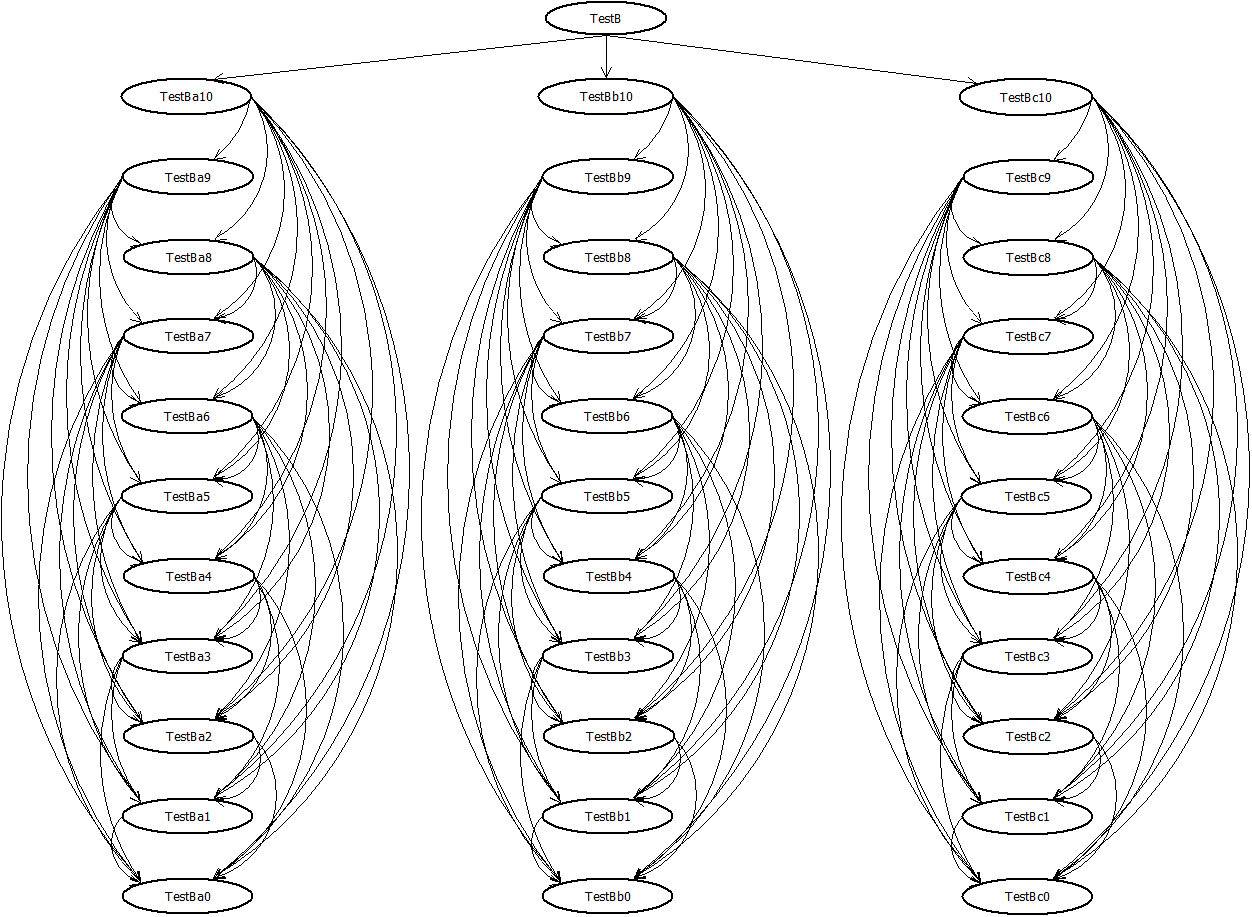
\includegraphics[width=\linewidth]{TestB.png}
  		\caption{Graf zależności dla testu B.}
  		\label{fig:testB}
	\end{center}
\end{figure}

Łatwo wywnioskować z Rys. \ref{fig:testB}, że tworząc obiekty poszczególnych typów ilość tworzonych obiektów rośnie ponad dziesięciokortnie:
\begin{itemize}
	\item typy od TestB00 do TestB09 - 1 obiekt,
	\item typy od TestB10 do TestB19 - 11 obiektów (obiekt danego typu plus 10 obiektów typów od TestB00 do TestB09),
	\item typy od TestB20 do TestB29 - 111 obiektów (obiekt danego typu plus 10 obiektów typów od TestB10 do TestB19),
	\item typy od TestB30 do TestB39 - 1 111 obiektów,
	\item  typy od TestB40 do TestB49 - 11 111 obiektów,
	\item TestB - 111 111 obiektów.
\end{itemize}
Zatem tworząc obiekt typu TestB, tworzymy: 1 obiekt typu TestB, 10 obiektów typów od TestB40 do TestB49, 100 obiektów typów od TestB30 do TestB39, 1 000 obiektów typów od TestB20 do TestB29, 10 000 obiektów typów od TestB10 do TestB19, 100 000 obiektów typów od TestB00 do TestB09.

\subsubsection{Wyniki dla Singleton}
Najlepiej poradziły sobie najpopularniejsze kontenery - Windsor i Aurofac. Kontener NiquIoCPartial uplasował się na 3 miejscu. Najsłabiej poradził sobie kontroler StructureMap i Unity.

\subsubsection{Wyniki dla Transient}
W tym teście ważne są nie tylko poszczególne czasy, ale jak i również wzrostu czasu wykonania wraz ze wzrostem ilości operacji.\\
Gdy mamy tylko 1 operację najlepiej radzi sobie NiquIoCPartial. Czasy pozostały są znacząco większe. Najsłabiej poradziły sobie DryIoc i NiquIoCFull.\\
Gdy mamy 10 operacji znacząco najlepiej radzi sobie SimplyInjector i NiquIoCPartial. Czołówkę zamykają StrucutreMap i NiquIoCFull. Pozostałe kontenery miały podobne, dużo słabsze czasy.\\
Warto tutaj zaznaczyć, że najmniejszy wzorst czasu miały kontenery SimpleInjector, NiquIoCFull, LightInject, DryIoc oraz Grace.

\subsubsection{Wyniki dla PerThread}
Czasy dla tego przypadku powinny być zbliżone do czasów dla Singleton, ponieważ wszystko było uruchamiane w jednym wątku, więc powinno się zachowywać jak singleton. Niestety prawie połowa kontenerów sobie z tym nie poradziła. Czasy zbliżone do czasów dla Singletona posiadają jedynie: Autofac, Ninject, NiquIoCPartial, NiquIoCFull, StructureMap, Unity i Windsor. Czasy dla pozostałych kontrolerów są od kilka do nawet kilkadziesiąt razy większe niż dla Singleton. Operacje dla kontenera LightInject działały tak długo (ponad 20 minut), że ich czas został zamieniony na -1.\\
Tak samo jak w przypadku Signleton najlepiej poradziły sobie najpopularniejsze kontenery - Windsor i Aurofac. Kontener NiquIoCPartial uplasował się na 3 miejscu. Najsłabiej poradził sobie kontroler LightInject i DryIoc.


\subsection{Przypadek testowy C}
\subsubsection{Opis}
Ten test jest bardzo podobny do test A, tylko dochodzi nam 1 dodatkowy poziom, który wygląda trochę inaczej. W głównym obiekcie "TestC" konstruktor przyjmuje 3 parametry następujących typów: "TestCa10", "TestCb10", "TestCc10". Każdy z tych 3 typów odpowiada typowi "TestA", więc przyjmuje on w konstruktorze 10 parametrów. Dla "TestCa10" są to parametry typów od "TestCa0" do "TestCa9", dla "TestCb10" są to parametry typów od "TestCb0" do "TestCb9", a dla "TestCc10" są to parametry typów od "TestCc0" do "TestCc9".\\

\begin{figure}[h]
	\begin{center}
  		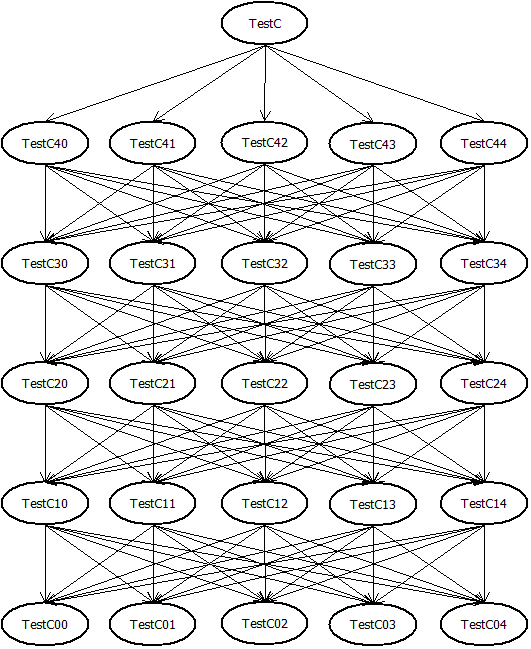
\includegraphics[width=\linewidth]{TestC.png}
  		\caption{Graf zależności dla testu C.}
  		\label{fig:testC}
	\end{center}
\end{figure}

Łatwo wywnioskować z Rys. \ref{fig:testC}, że tworząc obiekty poszczególnych typów ilość tworzonych obiektów rośnie dwukrotnie tak jak dla testu A:
\begin{itemize}
	\item TestCa0 - 1 obiekt,
	\item TestCa1 - 2 obiekty (obiekt typu TestCa1 i obiekt typu TestCa0),
	\item TestCa2 - 4 obiekty (obiekt typu TestCa2, obiekt typu TestCa1 - 2 obiekty, obiekt typu TestCa0 - 1 obiekt),
	\item TestCa3 - 8 obiektów (obiekt typu TestCa3, obiekt typu TestCa2 - 4 obiekty, obiekt typu TestCa1, obiekt typu TestCa0),
	\item TestCa4 - 16 obiektów,
	\item TestCa5 - 32 obiektów,
	\item TestCa6 - 64 obiektów,
	\item TestCa7 - 128 obiektów,
	\item TestCa8 - 256 obiektów,
	\item TestCa9 - 512 obiektów,
	\item TestCa10 - 1 024 obiektów,
	\item \ldots (dla TestCb i TestCc sytuacja wygląda dokłądnie tak samo jak dla TestCa),
	\item TestC - 3 073 obiektów.
\end{itemize}
Zatem tworząc obiekt typu TestC, tworzymy: 1 obiekt typu TestC, 1 obiekt typu TestCa10, TestCb10 i TestCc10,1 obiekt typu TestCa9, TestCb9 i TestCc9, 2 obiekty typu TestCa8, TestCb8 i TestCc8, 4 obiekty typu TestCa7, TestCb7 i TestCc7, 8 obiektów typu TestCa6, TestCb6 i TestCc6, 16 obiektów typu TestCa5, TestCb5 i TestCc5, 32 obiektów typu TestCa4, TestCb4 i TestCc4, 64 obiektów typu TestCa3, TestCb3 i TestCc3, 128 obiektów typu TestCa2, TestCb2 i TestCc2, 256 obiektów typu TestCa1, TestCb1 i TestCc1, 512 obiektów typu TestCa0, TestCb0 i TestCc0.

\subsubsection{Wyniki dla Singleton}
Najlepiej poradziły sobie najpopularniejsze kontenery - Windsor i Aurofac. Kontener NiquIoCPartial uplasował się na 3 miejscu. Najsłabiej poradził sobie kontroler StructureMap i Unity.

\subsubsection{Wyniki dla Transient}
W tym teście ważne są nie tylko poszczególne czasy, ale jak i również wzrostu czasu wykonania wraz ze wzrostem ilości operacji.\\
Gdy mamy tylko 1 operację najlepiej radzi sobie Autofac, a zaraz za nim NiquIoCPartial i Windsor. Najsłabiej DryIoc i SimplyInjector.\\
Gdy mamy 10 operacji znacząco najlepiej radzi sobie NiquIoCPartial (ponad dwa razy lepiej niż drugi Autofac). Kolejne miejsca należą do NiquIoCFul i LightInjectl. Pozostałe kontenery miałby podobne, dużo słabsze czasy. Najgorzej poradził sobie Ninject, który czas miał ponad 5 razy większy niż kontener z przedostatnim czasem (Grace).\\
Gdy mamy 100 operacji na prowadzenie wysuneły się mniej popularne kontenery, które prawdopodobniej mają najlepsze cachowanie. Kolejne miejsca to: NiquIoCFull, LightInject i SimpleInjector. Najsłabiej w tym przypadku poradziłysobie Ninject, Windsor, Unity i Autofac.\\
Dla przypadku z 1000 operacji do czołówki dołączył DryIoc (czasy zbliżone do SimpleInjector). Na pierwszym miejscu wciąż pozostaje NiquIoC. Pozostałe kontenery mają czasy od kilka do kilkanaście razy gorsze.\\
Warto tutaj zaznaczyć, że najmniejszy wzorst czasu miały kontenery NiquIoCFull, LightInject, DryIoc, SimpleInjector oraz Grace.

\subsubsection{Wyniki dla PerThread}
Czasy dla tego przypadku powinny być zbliżone do czasów dla Singleton, ponieważ wszystko było uruchamiane w jednym wątku, więc powinno się zachowywać jak singleton. Niestety prawie połowa kontenerów sobie z tym nie poradziła. Czasy zbliżone do czasów dla Singletona posiadają jedynie: Autofac, Ninject, NiquIoCPartial, NiquIoCFull, StructureMap, Unity i Windsor. Czasy dla pozostałych kontrolerów są od kilka do nawet kilkadziesiąt razy większe niż dla Singleton. Operacje dla kontenera LightInject działały tak długo (ponad 20 minut), że ich czas został zamieniony na -1.\\
Tak samo jak w przypadku Signleton najlepiej poradziły sobie najpopularniejsze kontenery - Windsor i Aurofac. Kontener NiquIoCPartial uplasował się na 3 miejscu. Najsłabiej poradził sobie kontroler LightInject i DryIoc.



\clearpage

\section{Podsumowanie}
<parę słów na koniec>

\newpage
\begin{thebibliography}{authordate1}
\bibitem{dependency_injection} Dependency Injection in .NET, Mark Seemann (str. 4-5)
\bibitem{emit} Expert .NET 2.0 IL Assembler, Serge Lidin (str. 3-7)
\end{thebibliography}

\end{document}